\documentclass{../lab_class}

\usepackage{fancyhdr}
\pagestyle{fancy}
\rhead{П.\,Ю. Смирнов, 687 гр.}
\lhead{Лабораторная работа № 4.3.5, МФТИ, весна 2018}

\begin{document}

{\Large 4.3.5 -- Изучение голограммы.}

\paragraph{Цель работы.}
Изучить свойства голограмм точечного источника и объёмного предмета.

В работе используются: гелий-неоновый лазер, голограммы, набор линз, предметная шкала, экран, линейка.

\paragraph{Теоретическая часть.}
Приёмники света реагируют лишь на интенсивность света, потому на фотопластинке информация о фазе падающей волны теряется. Голография есть способ записи полного портрета (и амплитуды, и фазы) волны. Для этого на фотопластинку помимо света от предмета падает \emph{опорная волна} известной амплитуды и фазы. Обе волны когеренты, благодаря чему мы можем наблюдать интерференцию на пластинке и по ней восстановить характеристики предметной волны. 

Голограмма Габора -- изображение точечного источника. Пусть такой источник создает сферическую волну $a/r \exp e^{ikr}$, опорная волна -- плоская волна $a \exp ikz$. Пусть амплитуда волн на пластинке $\simeq a$, а фаза равна нулю. Тогда квадрат амплитуды даётся выражением
\begin{equation*}
	I \sim 2a^2 + a^2 e^{-ikz} + a^2 e^{ikz}.
\end{equation*}
Первое слагаемое суть плоская волна, третье -- сферическая волна, дающая мнимое изображение предмета (голограммы), второе -- сферическая волна, дающая действительное изображение предмета (с другой стороны пластинки). 

Пусть пластинка расположена в плоскости $z = 0$. Обозначим расстояние до начала координат $\rho = \sqrt{x^2 + y^2}$. Тогда приближенно $r \simeq z_0 + \rho^2 / 2z_0$, где $z_0$ -- расстояние до предмета. Считая фазу волн на пластинке равной нулю, получаем $\varphi = \frac{k}{2z_0} \rho^2$. Отсюда для интенсивности света на пластинке получаем выражение
\begin{equation*}
	I(\rho) = 2a^2 \left( 1 + \cos \frac{k\rho^2}{2z_0} \right).
\end{equation*}
Мы видим, что интерференционная картина (наз. \emph{зонная решетка Габора}) имеет вид колец, центр которых находится в начале координат. Их радиус даётся выражением
\begin{equation}\label{eq:main}
	\rho = \sqrt{m \lambda z_0}.
\end{equation}

\paragraph{Эксперимент.}

\begin{figure}[H]
\centering
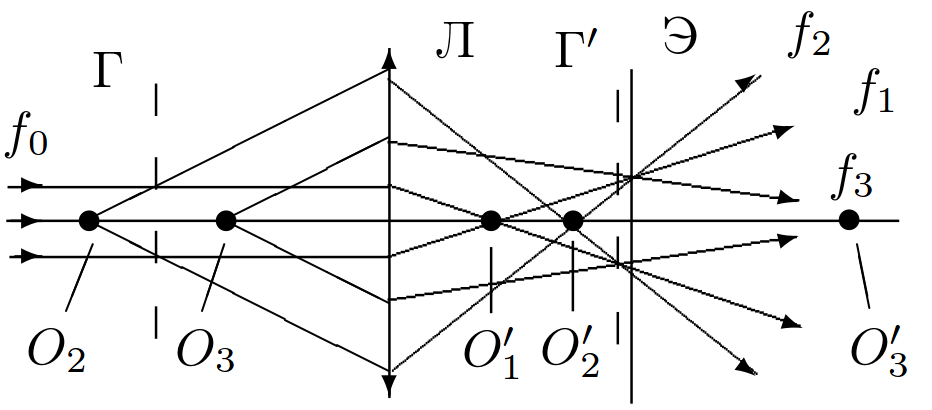
\includegraphics[width = 0.4 \textwidth]{sch01.png}
\caption{Схема установки}
	\label{fig:scheme}
\end{figure}

В работе используется гелий-неоновый лазер с длиной волны $\boxed{\lambda = 532 \ \sn \m}$. Цену деления предметной шкалы определяем по известной формуле для дифракции Фраунгофера $\lambda/D = \Delta x / L$. Имеем расстояние между дифракционными максимумами и расстояние между экраном и кассетой
\begin{gather*}
	\Delta x = 5.5 \ \cm, \\
	L = 118 \ \cm
\end{gather*}
соответственно. Отсюда $\boxed{D = 11.4 \ \smu \m}$.

Теперь осветим лазером голограмму. Дифракционное изображение на экране суть кольца, по радиусы которых (формула \ref{eq:main}) мы можем узнать расстояние до мнимого источника (до источника при записи голограммы при отс. увеличения) $z_0$. Имеем
\begin{equation*}
	\Delta\rho_1 = 1.5 \ \mm, \quad \Delta\rho_2 = 1.5 \ \mm, \quad \Delta\rho_3 = 1.8 \ \mm, \quad \Delta\rho_4 = 2.0 \ \mm,
\end{equation*}
откуда $z_0 \simeq 48.8 \ \m$ -- расстояние до мнимого источника. Расстояние же до источника при записи голограммы, как можно ожидать из воспоминаний о расположении линзы на установке, есть $d \simeq 48.8 \ \cm$.

В следующем опыте мы изучаем фокусирующие свойства самой голограммы, играющей роль короткофокусной линзы. Ранее мы уже нашли цену деления предметной шкалы $D$. Теперь подвинем её вплотную к голограмме. Расстояние от экрана до голограммы $b = 45.5 \ \cm$, наблюдаемое расстояние между штрихами на экране $D' = 2 \ \mm$. Отсюда получаем фокусное расстояние голограммы $f \simeq 45.8 \ \cm = d$. Полученный результат согласуется с другим методом, использованным выше. 

На нашу голограмму записано не абы что, а изображение самой настоящей трёхмерной линейки! Используя способность головы к вращению, получаем, что опорная волна при записи голограммы падала на предмет под углом порядка $\simeq 5^{\circ}$.

\paragraph{Вывод.}
Мы изучили основные свойства голограммы точечного источника и были удивлены открытием Габора. 

\end{document}